
{\color{blue} Набирала Белла 36-42. Есть вопросы, выделены жирным, кое-что не нашла вовсе.}
\begin{notation} 
Модель в факторном анализе имеет вид

\begin{gather}\label{eq:model}
\xi = \mathbb{F}\mathbb{\eta} + \mathbb{\eps},
\end{gather}
где

\begin{enumerate}

\item

$\xi$ --- исходный вектор признаков.
\item
$\mathbb{F} = [F_1:\ldots:F_r] = \{f_{ij}\} \in \mathbb{R}^{p\times r}$ --- матрица факторных нагрузок.

\item
$\mathbb{\eta} \in \mathbb{R}^{r}$ --- факторное значение.

\item 
$\mathbb{\eps} \in  \mathbb{R}^{p}$ --- вектор индивидуальных (характерных/специфических) факторов {\bf{(можно ли так говорить?)}}.

\item
$p$ --- исходное число признаков, $r$ --- число общих факторов \bf{(можно ли так говорить?)}, $r << p$.

\end{enumerate}

Предполагаемые условия:

\begin{enumerate}
\item 
$\mathbb{E}\mathbb{\eta} = 0, 
\ \mathbb{D}\mathbb{\eta}= 1, 
\ \eta_{i}$ --- некорр.

\item 
$\mathbb{\eps}$ и $\mathbb{\eta}$ некорр., $\eps_{i}$ некорр. между собой.


\item
$\mathbb{E}\mathbb{\eps} = 0, 
\ {\rm cov}(\eps) = {\rm diag}(\sigma_1^2,..,\sigma_p^2),
\ {\rm cov}(\xi) = \Sigma, 
\ \tilde\xi = \mathbb{F}\mathbb{\eta}, 
\ {\rm cov}(\mathbb{\eps}) = {\Psi},
\ {\rm cov}(\tilde\xi) = \mathbb{FF^\mathrm{T}}$
\end{enumerate}

Модель \eqref{eq:model} переписывается как  $\Sigma = \mathbb{FF^\mathrm{T}} + \Psi$,

$\xi_{i} = f_{i1}\eta_1 +\cdots+f_{ir}\eta_r + \eps_i$.
\end{notation}

\begin{note}
  Почти всегда предполагается, что признаки стандартизованы, то есть ${\rm cov}(\xi) = {\rm corr}(\xi)$.
\end{note}

\subsection{ 36. Какая разница между АГК и факторным анализом?}

\begin{enumerate}
\item
В факторном анализе есть модель.

\item
В факторном анализе не может быть факторов, которые уникальны по одному признаку, то есть  $F_i$ не может иметь вид $
\begin{pmatrix}
  0 \\
  0 \\
  \vdots \\
  a \\
  0
\end{pmatrix}$. Такие факторы относятся к уникальным, то есть входят в $\eps$, а мы интересуемся общей частью.
\end{enumerate}


\subsection{ 37. Связь между числом факторов и числом признаков для корректности задачи.}

Из $\Sigma = \mathbb{FF^\mathrm{T}} + \Psi$ получаем $\frac{p(p+1)}{2}$ равенств (помним, что $\Sigma$ --- симметр.) и \\ число~параметров~$\leq pr+p$.

Условие корректности задачи $pr+p \leq \frac{p(p+1)}{2} \Rightarrow r \leq  \frac{p-1}{2}$.

Получили условие, когда число уравнение не меньше числа параметров. Тут была заминка на лекции (2015.X.08), примерно 40-50 минута .  Сошлись на том, что если модель верна, то лишние уравнения не сделают ее неверной. Если бы знак стоял в обратную сторону, то вышло бы, что равенства модель не характеризуют.

\subsection{ 38. Что минимизируется в методе MINRES? В чем разница с тем, что минимизируется в АГК?}

Задача на выборочном языке имеет вид $\mathbb{X} = \mathbb{VF^\mathrm{T}} + \mathbb{\eps}$, где $\mathbb{X} \in \mathbb{R}^{n\times p}, 
\ \mathbb{V} \in \mathbb{R}^{n\times r},
\ \mathbb{F} \in \mathbb{R}^{p\times r}$.

Пусть $\mathbb{S}$ --- выборочная ковариационная матрица (известна). $\parallel \mathbb{S} - (\mathbb{FF^\mathrm{T}} + \Psi)\parallel^2_F \rightarrow \min\limits_{\mathbb{F},\Psi}$ (Метод Наименьших Квадратов).

Пусть $\tilde{\mathbb{S}} := \mathbb{FF^\mathrm{T}} + \Psi$. Тогда $\sum\limits_{i,j}(S_{ij} - \tilde S_{ij})^2 \rightarrow \min$.


\begin{gather*} 
\begin{cases}
 \sum\limits_{i\neq j}(S_{ij} - \sum\limits_{k = 1}^r f_{ik}f_{jk})^2 \rightarrow min,\\ 
(\mathbb{FF^\mathrm{T}})_{ii} \leq 1 \Rightarrow \sigma_i^2 = 1 - (\mathbb{FF^\mathrm{T}})_{ii}.
\end{cases}
\end{gather*}

Minres --- minimization residual correlations (минимизация разницы известных корреляций и той их частью, что объясняется факторами).

АГК: $\parallel \mathbb{Y} - \mathbb{\tilde{Y}} \parallel \rightarrow \min\limits_{rank\mathrm{\tilde{Y}} \leq r} \Leftrightarrow \parallel \mathbb{Y}\mathbb{Y}^\mathrm{T} - \tilde{\mathbb{Y}} \tilde{\mathbb{Y}}^\mathrm{T} \parallel  
\rightarrow \min\limits_{rank\mathrm{\tilde{Y}} \leq r}$

 {\bf{Тут надо все пояснить про АГК, но меня не было на лекции той, простите-помогите.}}
\subsection{ 39. Какой вид имеет функция правдоподобия в ФА?}

Пусть $\xi \sim N(0, \Sigma)$.

$\mathcal{L}(\mathbb{X};\mathbb{F}, \Psi) = \prod\limits_{i =1}^n \frac{1}{(2\pi)^{n/2}\det{\Sigma}^{1/2}} e^{-\frac{1}{2}X_i^\mathrm{T}\Sigma^-1X_i} = \prod\limits_{i =1}^n \frac{1}{(2\pi)^{n/2}\det({\mathbb{FF^\mathrm{T}} + \Psi)}^{1/2}} e^{-\frac{1}{2}(X_i^\mathrm{T}(\mathbb{FF^\mathrm{T})} + \Psi^{-1})X_i}$.

Вместо  $\mathbb{X}$ рассм. выборочная ковар. матрица $\mathbb{S}$.
$\mathcal{L}(\mathbb{S};\mathbb{F}, \Psi)  \sim W_{p}(\Sigma)$.

Так как решений бесконечно много с точностью до вращений, и чтобы как-т о зафиксировать$\mathcal{L}(\mathbb{S};\mathbb{F}, \Psi) \rightarrow \max\limits_{\mathbb{F},\Psi}$
\subsection{ 40.  Проверка значимости модели ФА.}

{\bf{Не уверена, что это тот самый вопрос.}} \\
$H_{0}: \Sigma = \mathbb{FF^\mathrm{T}} + \Psi$ 

Статистика критерия $t = \left(n-1 - \frac{2p+4r-5}{6}\right)ln\left(\frac{|\mathbb{\hat{F_{ОМП}}\hat{F_{ОМП}}^\mathrm{T}+}+\hat{\Psi_{ОМП}}|}{|\mathrm{\hat{S}}|}\right) \sim \chi^2\left(\frac{(p+r)^2 - (p+r)}{2}\right)$.


\subsection{ 41.  Критерий сферичности Бартлетта, для чего нужен}


Частный случай критерия (Вопрос 40 ) при $r = 0$, имеет смысл проверять перед поиском факторов, вдруг общих факторов совсем нет.

$H_0: \Sigma =  \left(\begin{matrix}
1&\cdots& 0 \\
\vdots&1& \vdots \\
0&\cdots& 1
\end{matrix}\right)$ --- сферичность (т.к. данные выглядят как сфера).

Статистика критерия $t = \left(n-1 - \frac{2p-5}{6}\right)ln\left(\frac{1}{\mathbb{\hat{S}}}\right) \sim \chi^2\left(\frac{p^2 - p}{2}\right)$.

\subsection{ 42. Что такое общность и уникальность признака? Какие факторы не находит факторный анализ?}

$\sum\limits_{j = 1}^r{f_{ij}^2 = 1 - D(\eps_i)}$ --- communality(общность),  $D(\eps_i)$ --- уникальность.


\begin{ex}

	 \begin{figure}[h!]
	 	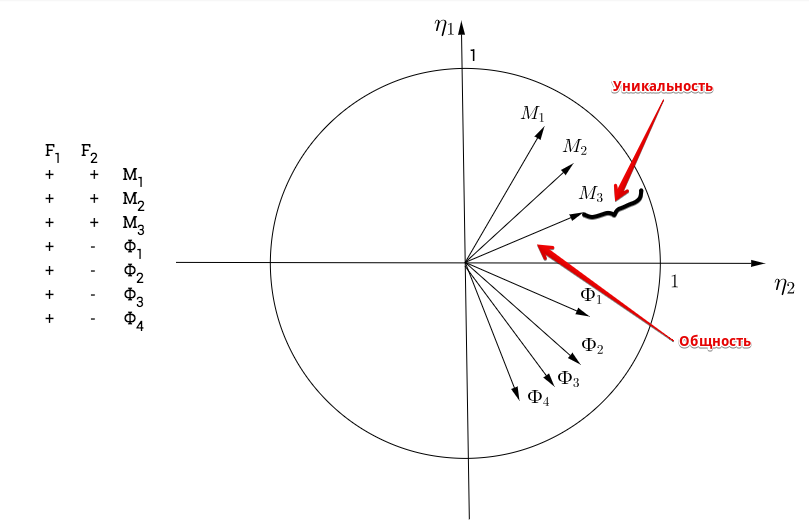
\includegraphics[scale=0.65]{img/Example.png}
	 \end{figure}
	
	
	При повороте осей примерно на $45^{\circ}$ получим скрытые факторы --- это способности по математике и по физике.
	
	{\bf{Не нашла материла про то, какие факторы не находит факторый анализ.}}
\end{ex}
